% Section content template for individual Educative lessons
% This file contains the actual content for a specific section
% Generated from Educative API section content

% Section: Detailed Design of a Monitoring System
% Section ID: 6718061809238016
% Section Slug: detailed-design-of-a-monitoring-system
% Generated: 2025-12-07T18:38:29.809448

We'll discuss the core components of our monitoring system, identify the shortcomings of our design, and improve the design to fulfill our requirements.

\subsection{Storage}\label{izgIMhnJTKTCELWCxvYkA}
\\
We'll use time-series databases to save the data locally on the server where our monitoring service is running. Then , we'll integrate it with a separate storage node. We'll use blob storage to store our metrics.
\\
We need to store metrics and know which action to perform if a metric has reached a particular value. For example, if CPU usage exceeds 90\%, we generate an alert to the end user so the alert receiver can take the necessary steps, such as allocating more resources to scale. For this purpose, we need another storage area that will contain the rules and actions. Let's call it a rules database. Upon any violation of the rules, we can take appropriate action.
\\
Here, we have identified two more components in our design---that is, a rules and action database and a storage node (a blob store).

\begin{figure}[htbp]
 \centering
 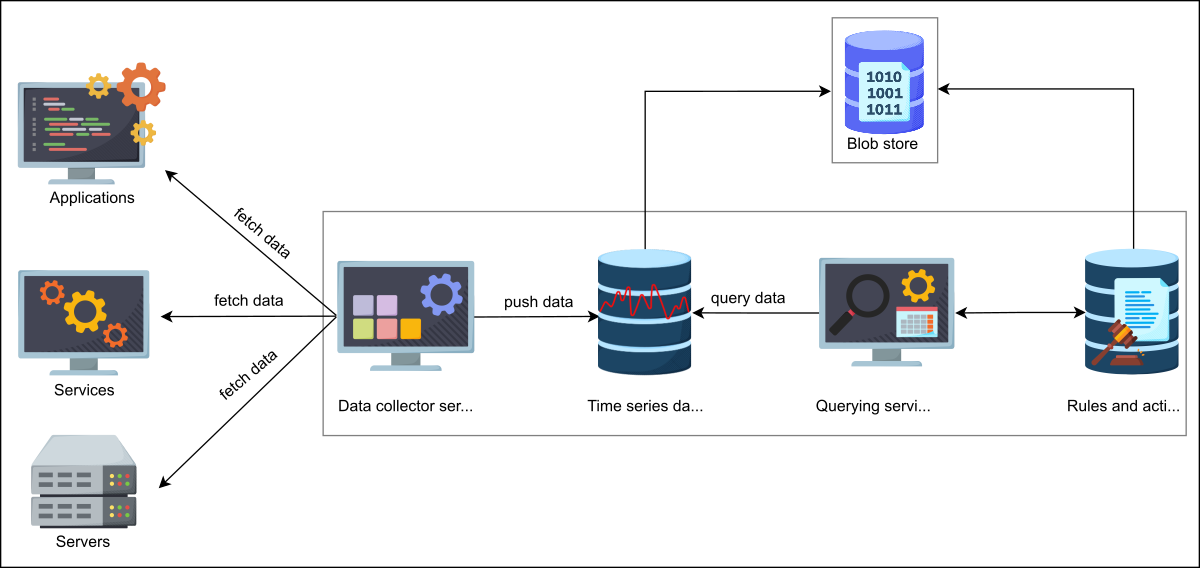
\includegraphics[width=0.5\textwidth]{Images/chapter_14/section_6718061809238016/6366277779456000.png}
 \caption{Adding blob storage and a rules and action database}
\end{figure}

\subsection{Data collector}\label{JrqjRgxLvxNoVZR-aHGiJ}
\\
We need a monitoring system to update us about our several data centers. We can stay updated if the information about our processes reaches us, which is possible through logging. We 'll choose a pull strategy. Then, we'll extract our relevant metrics from the logs of the application. As discussed in our logging design, we used a \href{https://www.educative.io/courses/grokking-the-system-design-interview/design-of-a-distributed-logging-service\#Using-distributed-messaging-queue}{distributed messaging queue}. The message in the queue has the service name, ID, and a short description of the log. This will help us identify the metric and its information for a specific service. Exposing the relevant metrics to the data collector is necessary for monitoring any service so that our data collector can get the metrics from the service and store them into the time-series database.
\\
A real-world example of a monitoring system based on the pull-based approach is DigitalOcean(DigitalOcean, Inc. is an American cloud infrastructure provider that allows developers to deploy and scale applications that run simultaneously on multiple computers.). It monitors millions of machines that are dispersed globally.

\begin{quote}
\textbf{Quiz:}
\textbf{Question 1:} What are some drawbacks of using a push-based approach?
\textbf{Answer:} The push-based monitoring tool collects metric data from the applications and servers and sends it to a central collection platform.

Each microservice sends its metrics to the monitoring system, resulting in a heavy traffic load on the infrastructure. This is how monitoring might become a bottleneck for business operations. The monitoring can be near real-time. However, if appropriate care isn't taken, it can overwhelm the infrastructure with continual push requests from all services, resulting in network floods. We must also install daemons on each of these targets to send metrics to the monitoring server, which requires additional work.
\end{quote}

\subsubsection{Service discoverer}\label{hGF6mGKY5pd5X77fO_KQC}
\\
The data collector is responsible for fetching metrics from the services it monitors. This way, the monitoring system doesn't need to keep track of services. Instead , it can find them using the discoverer service. We
'll save the relevant information about the services we have to monitor. We 'll use a service discovery solution and integrate with several platforms and tools, including EC2, Kubernetes, and Consul. This will allow us to discover which services we have to monitor. Similar dynamic discovery can be used for newly commissioned hardware.
\\
Let's add our newly identified component to our existing design.

\begin{figure}[htbp]
 \centering
 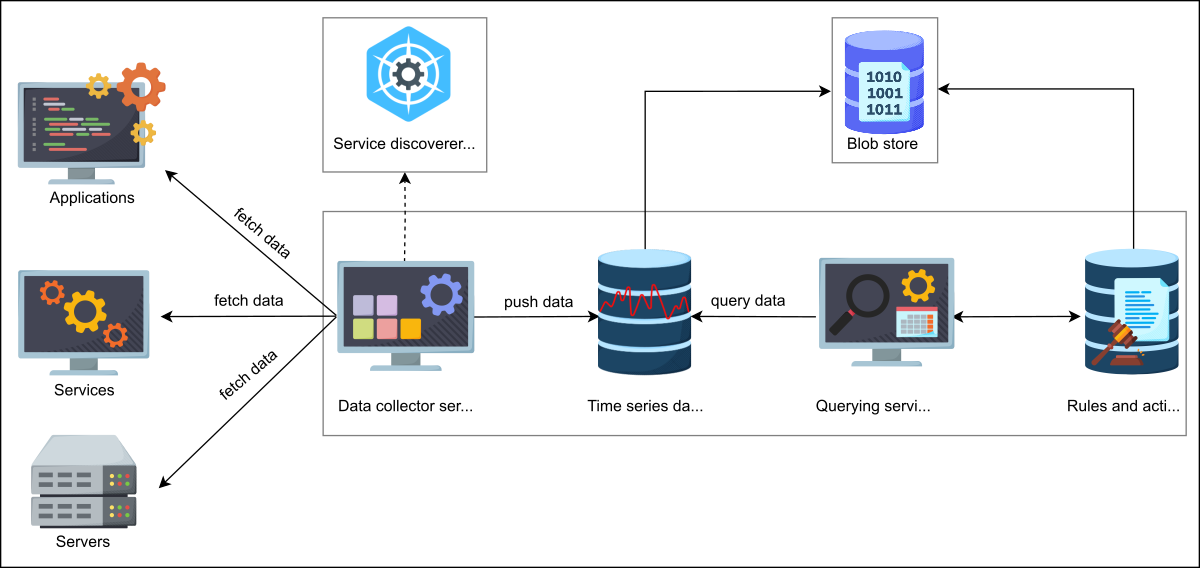
\includegraphics[width=0.5\textwidth]{Images/chapter_14/section_6718061809238016/5987402809475072.png}
 \caption{Adding the service discoverer}
\end{figure}

\subsection{Querying Service}\label{A4vTA-ZOfrzoTj7CPy6K3}
\\
We want a service to access the database and fetch the relevant query results. We need this because we want to view the errors like values of a particular node's memory usage, or send an alert if a metric exceeds the set limit. Let 's add the two components we need along with querying.

\subsubsection{Alert Manager}\label{tCW3Q-5NX_8WZHyl_ttLj}
\\
The alert manager is responsible for sending alerts upon violations of set rules. It can send alerts as an email, a Slack message, and so on.

\subsubsection{Dashboard}\label{m4G7pOgbDrffAGvwbaHGk}
\\
We can set dashboards by using the collected metrics to display the required information---for example, the number of requests in the current week.
\\
Let's add the components discussed above, which completes our design of the monitoring system.

\begin{figure}[htbp]
 \centering
 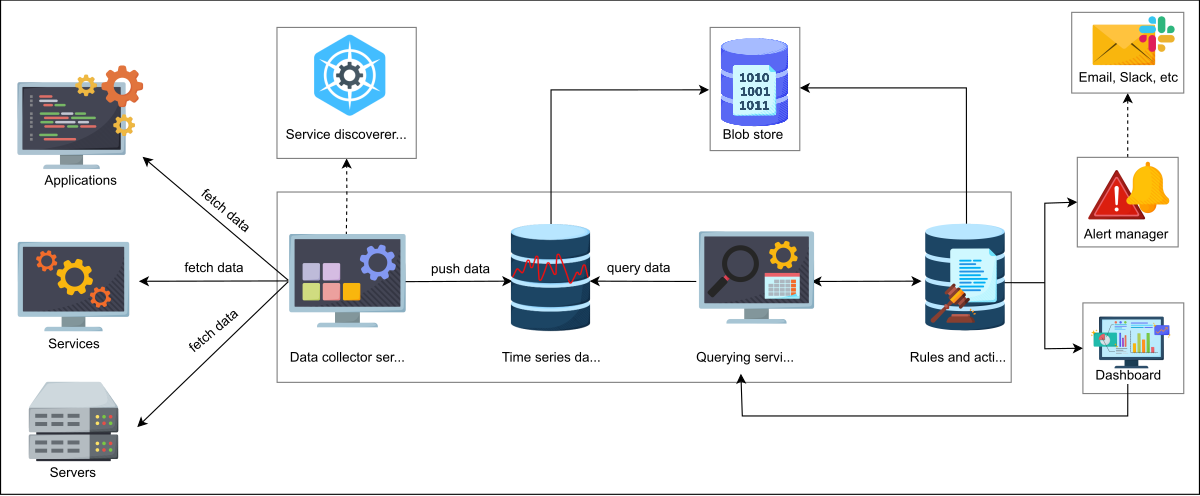
\includegraphics[width=0.5\textwidth]{Images/chapter_14/section_6718061809238016/6150343349370880.png}
 \caption{Detailed design of monitoring system}
\end{figure}

Our all-in-one monitoring service works for actively tracking systems and services. It collects and stores data, and it supports searches, graphs, and alerts.\\

\subsection{Pros}\label{lLWzEoYw0sd6VHUk_GMhg}

\begin{itemize}
\item
\protect\phantomsection\label{OizYJYEafwPjpaR4KcEQC}
The design of our monitoring service ensures the smooth working of the operations and keeps an eye on signs of impending problems.
\item
\protect\phantomsection\label{GXlOlhzTIpw9OKMfgw65N}
Our design avoids overloading the network traffic by fetching the data itself.
\item
\protect\phantomsection\label{X3jvtjAaVcJXUMLATzH1V}
The monitoring service provides higher availability.
\end{itemize}

\subsection{Cons}\label{rJQ3FGmRAhwT16rgsfC_m}

\begin{itemize}
\item
\protect\phantomsection\label{vhYCBtVMIp3E7t-wIYJRM}
The system seems scalable, but managing more servers to monitor can be a problem. For example, we have a dedicated server responsible for running the monitoring service. It can be a single point of failure (SPOF). To cater to SPOF, we can have a failover server for our monitoring system. Then , we also need to maintain consistency between actual and failover servers. However, such a design will also hit a scalability ceiling as the number of servers further increase.
\item
\protect\phantomsection\label{WPwl7tfM7L5DaJRPKkZWG}
Monitoring collects an enormous amount of data 24/7, and keeping it forever might not be feasible. We need a policy andmechanisms to delete unwanted data periodically to efficiently utilize the resources.
\end{itemize}
\\
Let's think of a way to overcome the problems with our monitoring service.

\subsection{Improving our design}\label{AeZ91Rtz_Jlk-uD_hFaUw}
\\
\hfill\break
We want to improve our design so that our system can scale better and decide what data to keep and what to delete. Let 's see how the push-based approach works. In a push-based approach, the application pushes its data to the monitoring system.

\begin{figure}[htbp]
 \centering
 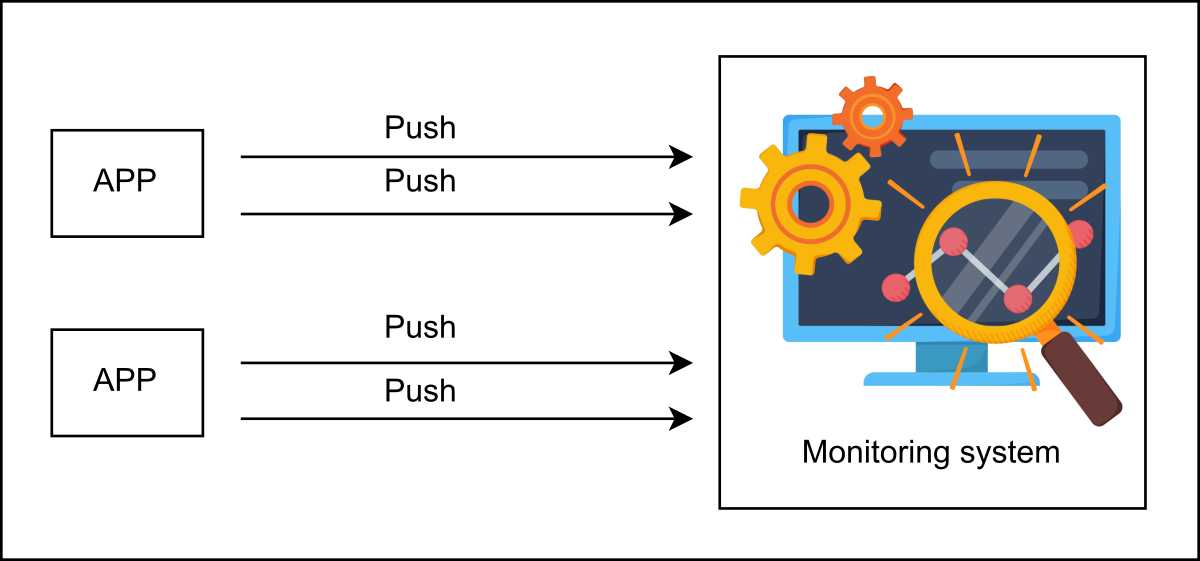
\includegraphics[width=0.5\textwidth]{Images/chapter_14/section_6718061809238016/6089376624148480.png}
 \caption{Push-based monitoring system}
\end{figure}

We used a pull-based strategy to avoid network congestion. This also allows the applications to be free of the aspect that they have to send the relevant monitoring data of to the system. Instead , the monitoring system fetches or pulls the data itself. To cater to scaling needs, we need to apply a push-based approach too. We
'll use a hybrid approach by combining our pull-based strategy with the push-based strategy.
\\
We'll keep using a pull-based strategy for several servers within a data center. We 'll also assign several monitoring servers for hundreds or thousands of servers within a data center---let's say one server monitoring 5,000 servers. We
'll call them secondary monitoring servers.
\\
Now, we'll apply the push-based strategy. The secondary monitoring systems will push their data to a primary data center server. The primary data center server will push its data to a global monitoring service responsible for checking all the data centers spread globally.
\\
We'll use blob storage to store our excessive data, apply elastic search, and view our relevant stats using a visualizer. As our servers or data centers increase, we'll add more monitoring systems. The design for this is given below.
\begin{quote}
\textbf{Note}: Using a hierarchy of systems for scaling is a common design pattern in system design. By increasing nodes on a level or introducing additional levels in the hierarchy, we get the ability to scale according to our current needs.
\end{quote}

\begin{figure}[htbp]
 \centering
 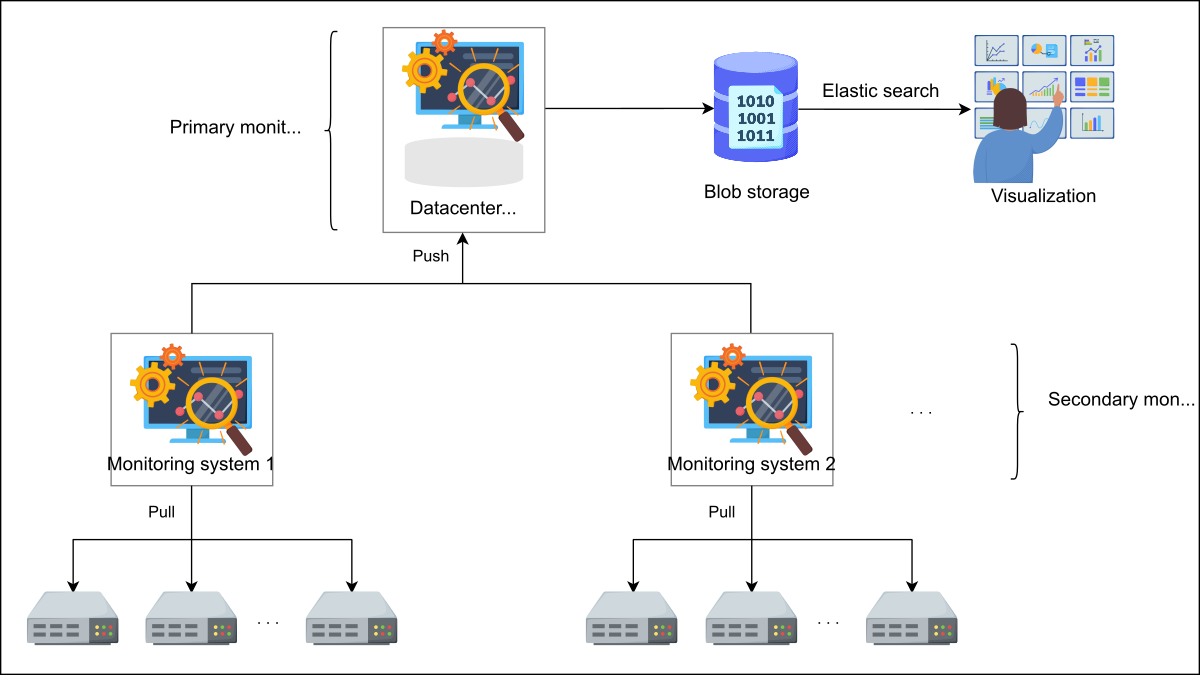
\includegraphics[width=0.5\textwidth]{Images/chapter_14/section_6718061809238016/6363563343347712.png}
 \caption{Adding the service discoverer}
\end{figure}

\begin{quote}
\textbf{Quiz:}
\textbf{Question 1:} What happens if a local or global monitoring system is down?
\textbf{Answer:} We can store the data locally and wait for the system to be up and running again. But there's a limit for the local data storage. So,

either we delete previous data or we don't store new data. To make a decision, relevant policies need to be created.
\textbf{Question 2:} How can a monitoring system reliably work if it uses the same infrastructure in a data center that it was supposed to monitor?

Consider this given that a failure of a network in a data center can knock out the monitoring components.
\textbf{Answer:} The actual deployment of a monitoring system needs special care. We might have an internal, monitoring-specific network to isolate it from the common network. We should use a separate instance of blob stores and other services. It also helps to have external components to the monitoring, where external might mean an independent service provider's infrastructure. However, designing such a system is complex and is more expensive.
\end{quote}

Humans need to consume enormous amounts of data, and even after different kinds of data summarizations, the data can still be huge. Next , we'll tackle how to present enormous data to human administrators.

% End of section content